\section{Two lateral stationary actions}\label{sec:arrays}

For the tangent section fixed in \Cref{sec:geometry}, use the normalized
family and its polynomial-growth jets from Proposition~\ref{lin:family}.
The reduced coordinates are \(p=(b,x)\),
and the compact observation values are \(q=\mathsf P(p)\), with
invertible Jacobian \(J=D_p\mathsf P\).  A normalized surface has
compact-source multiplier \(\lambda\).  Thus its interior first
variation is \(\lambda\cdot dq\), and the formal action satisfies
\[
 d\mathcal F(p)=\lambda_{\mathrm{formal}}\cdot d\mathsf P(p),
 \qquad \nabla_p\mathcal F=J^{\mathsf T}\lambda_{\mathrm{formal}}.
\]
All pairings and induced metrics in the complex construction are
bilinear.  Square roots are continued from the positive real area
element.  The observation charts remain fixed on the support of the
observations.

Suppose, for a contradiction to the obstruction to be proved below,
that there is a real formal arc
\begin{equation}\label{arr:critical-arc}
 \widehat p(s)=(\widehat b(s),\widehat x(s)),\qquad
 \nabla\mathcal F(\widehat p(s))=0,\qquad
 \widehat x(s)=s^k v+O(s^{k+1}),\quad v\ne0,\quad k\ge1.
\end{equation}
Its center is \(0\).  Formal differentiation shows also that
\(\mathcal F(\widehat p(s))=\mathcal F(0)\).
Put \(a=s^k\), retaining a continuous argument of \(s\), and put
\(B=|a|^{-1/2}\).  There is no assertion of single-valuedness in \(a\).
Here \(\beta_j(b,x)\) is the first-jet opening coefficient,
homogeneous linear in \(x\) for fixed \(b\), with analytic
\(b\)-dependent coefficients.  The leading coefficients along the arc are
\(\beta_j(\widehat p(s))=c_j a+o(a)\), with \(c_j\in\mathbb R\).
At least one \(c_j\) is nonzero.

On a chosen evaluation ray, call an end \emph{adverse} when its
leading opening \(c_j a\) is negative real, so the circular profile
\(R_c(z)=\sqrt{2(1+\beta_j z^2)}\) reaches radius zero at a
positive leading squared height \(Z_{j,\mathrm{lead}}^2=(-c_j a)^{-1}\).
Nearby complex rays retain the same adverse end list.  On all these
rays define the positive leading action scale by
\begin{equation}\label{arr:A0}
 A_{\mathrm{lead}}
   =\min_{\mathrm{adverse}\ j}\frac{|Z_{j,\mathrm{lead}}|^2}{4}.
\end{equation}

The construction uses three actual objects.  Real stopped actions
$F_H$ are holomorphic on full shrinking parameter disks and identify
the Gaussian formal action through a telescoping estimate and the real
comparison above.  The two lateral actions $G_+$ and $G_-$ come from
normalized solves on opposite bypasses of the adverse zero radius.
Finally, regular implicit operations select parameters $p_+$ and $p_-$
that realize the formal critical constraints to exponential accuracy.
Endpoint comparison and Taylor transport put the two actions at one
common parameter, with the upper bound in \Cref{arr:action-upper}.
The collapsing-end calculation will give a conflicting lower bound.

Here is the order of the stationary choices.  Fix the arc and a
continuous argument of $s$; both lateral evaluations use the same
$s$-sheet.  When all nonzero $c_j$ are positive, the adverse evaluation
starts at $\arg s=\pi/k$, including even $k$.  Prescribe a finite
required accuracy $K$, then choose the contour constant $D$ sufficiently
large.  Its excess angle $\delta=\eta D^{-1/2}$ and strict margins are
held fixed as $s\to0$; a larger $K$ may require a new $D$.
The relevant statements are \Cref{arr:contours,arr:flatness-upgrade}
and \eqref{arr:arbitrary-flatness}.

\subsection{Strict contours and their homotopies}\label{sec:contours}

The circular comparison profile on a cylindrical end is
\[
 R_c(z)=\sqrt{2(1+\beta z^2)}.
\]
After division by the drift coefficient, the leading radial and
angular diffusion coefficients on a parametrized path have positive
real parts precisely when, with fixed strict margins,
\begin{equation}\label{arr:path-signs}
 \operatorname{Re}d(z^2)>0,\qquad
 d\log\left|\frac{z^2}{1+\beta z^2}\right|>0.
\end{equation}
Indeed, with real path parameter \(\tau\), those coefficients are
\(D_r=2/(zz_\tau)=4/(z^2)_\tau\) and
\(D_\theta=2z_\tau/(zR_c^2)\).  The logarithmic derivative in
\eqref{arr:path-signs} is \(2\operatorname{Re}D_\theta\).
The exact circular axial-slope coefficients differ by \(O(B^{-2})\)
on fixed nondegenerate scaled bands, and preserve the strict signs.
These statements
concern the drift-normalized equation on a real parameter interval,
not continuation of unknown smooth spatial data.

\begin{lemma}[Admissible contour families]\label{arr:contours}
Fix the finite list of nonzero leading opening coefficients.  For
every sufficiently large fixed \(D\), there are upper and lower
families of contours on sectors of the \(a\)-cover containing,
respectively, the argument intervals \([0,\pi]\) and \([-\pi,0]\),
with excess angle
\(\delta=\eta D^{-1/2}\), where \(\eta>0\) is fixed sufficiently small.
The contours start on the real axis, satisfy
\eqref{arr:path-signs} strictly, avoid \(1+\beta z^2=0\), and end at
\(\operatorname{Re}z^2=D/|a|\).  They obey
\(|a||z|^2\le C_D\).
Their normalized derivatives and the inverse diffusion margins are
bounded by constants depending on \(D\).

The families can be chosen smooth in sector parameters.  As geometric
paths they admit shortening, deformation before an adverse pole to a
common real contour with endpoint at three quarters of the leading
squared pole height, and deformation beyond that pole to the height
turns used in the jump calculation.  The bounded scaled part of these
homotopies can be kept in \(|R_c|\ge r_*\) for a fixed \(r_*>0\).
The homothetic turns with shrinking \(|R_c|\) retain the displayed
geometric signs, but their solutions will be constructed in the separate
height norms of \Cref{sec:jump}.  Boundary data are specified by the
solve statements below, not by this geometric lemma.  These assertions
persist in sufficiently small polynomial-radius complex balls about
any fixed high-order polynomial approximation to \(\widehat p\).
\end{lemma}

\begin{proof}
Scale \(z^2\) by \(|a|\) and the absolute leading coefficient so that
the leading pole is \(p_*\), with \(|p_*|=1\).
For the lower bypass write \(u=h-iY(h)\), \(h'>0\), and choose real
\(c,d\) by
\(\operatorname{Re}(u/p_*)=ch+dY\); thus \(c^2+d^2=1\).
Put \(Q=h^2+Y^2\).  The exact identity
\[
 \frac{|u-p_*|^2}{|u|^2}
   =1-2H,\qquad H=\frac{ch+dY-\tfrac12}{Q},
\]
shows that the second condition in \eqref{arr:path-signs} is \(H'>0\).
Direct differentiation gives
\begin{equation}\label{arr:contour-numerator}
 Q^2H'=N=cA+dJ+h+YY',\quad
 A=Y^2-h^2-2hYY',\quad J=(h^2-Y^2)Y'-2hY.
\end{equation}
The first condition is simply \(dh>0\).

Near the adverse direction let \(e=4\delta\), \(0<e\le0.1\),
and take the positive branch
\[
 |d|\le e/2,\qquad c=\sqrt{1-d^2}\ge\sqrt{1-e^2/4}.
\]
Join the origin to
\((h_0,Y_0)=(1/4,\,0.6/e)\) by the ray \(Y=mh\),
\(m=2.4/e\).  On this ray
\[
 N=(1+m^2)h\{1-(c+dm)h\}.
\]
For \(c\le1\) and \(|d|\le e/2\), its worst endpoint projection is
\(1/4+0.3=0.55<1\).
From \((h_0,Y_0)\) follow the larger positive root of
\begin{equation}\label{arr:circle}
 K(h^2+Y^2)=h+eY-\tfrac12,\qquad
 K=\frac{0.35}{0.0625+0.36/e^2}.
\end{equation}
Here \(0.970<K/e^2<0.973\), and
\[
 Y'=\frac{1-2Kh}{2KY-e}>0
 \quad\hbox{for }\quad 1/4\le h\le0.01/e^2.
\]
The denominator is positive at the starting point and remains
positive on this branch.  If \(h\le1\), then \(Y\ge0.6/e\ge6>h\).
If \(h\ge1\), the circle identity implies
\[
 KY^2\ge h-\tfrac12-Kh^2\ge0.49h,\qquad
 \frac Yh\ge\sqrt{\frac{0.49}{Kh}}>7.
\]
Consequently \(J<0\).  The circle has \(N(1,e)=0\); eliminating \(A\)
from \eqref{arr:contour-numerator} gives the decisive exact identity
\begin{equation}\label{arr:circle-strict}
 N(c,d)=(1-c)(h+YY')+(d-ce)J>0.
\end{equation}
Both terms are nonnegative and the second is positive, since
\(ce>d\).  Thus a level circle for the auxiliary parameters gives
strict increase for every actual pole parameter under consideration.

If the absolute nonzero leading coefficients are \(b_j>0\), the
required horizontal endpoint is \(h=b_jD\).  The choice
\[
 16\eta^2\max_j b_j<0.01
\]
places every such endpoint in the circle interval.  This proves the
claimed \(D^{-1/2}\) angular reach.  Constants such as the imaginary
height are allowed to depend on the now fixed \(D\).

We give the blending argument, since endpoints alone do not suffice
for subsequent action comparisons.  On the circle define
\[
 Q_c=cY^2+(1-2ch)YY'.
\]
Equation \eqref{arr:circle} gives
\[
 Q_1=\frac{Y\{eY+2Kh(h-1)\}}{2KY-e}>0,\qquad
 Q_c=cQ_1+(1-c)YY'>0.
\]
For \(h\le1\), use \(eY\ge0.6\) and
\(2Kh(h-1)\ge-K/2\); for \(h\ge1\) positivity is immediate.
At \(d=0\), replacing \(Y\) by \(tY\), \(t\ge1\), changes the numerator
to \(h(1-ch)+t^2Q_c\), which is positive at \(t=1\) and increases.
On the favorable overlap \(d\le-\delta/2\), the extra contribution
\(dJ_t\) is positive.  Hence arbitrary fixed magnification of \(Y\)
preserves admissibility.
On a fixed compact interval write a magnified profile as \(Y=Mf(h)\).
Interpolate \(f\) to a positive increasing ray profile, keeping both
\(f\) and \(f'\) bounded below.  The favorable contribution is
\[
 |d|M^3f^2f'+O(M),
\]
while the remaining terms are \(O(M^2)\).  A sufficiently large
fixed \(M\) makes the entire interpolation admissible.  Initial
pieces may already be rays.  Away from the adverse direction, a ray
with \(\operatorname{Re}du>0\) and
\(\operatorname{Re}(u/p_*)<0\) works: for
\(p_*=e^{i\varphi}\), \(0<\varphi<\pi\), take
\(u=h(1-im)\) with \(\cos\varphi-m\sin\varphi<0\).
This joins the favorable overlap.  Reflection supplies the other
family.  At every join the strict conditions are linear in the
tangent vector at the point, so smoothing corners preserves them.
Near \(u=0\) the logarithmic condition reduces to increasing modulus,
and the start can be made real.

For a real leading adverse pole, set \(V=Y^2\).  Formula
\eqref{arr:contour-numerator} becomes
\begin{equation}\label{arr:affine-homotopy}
 N(V)=h(1-h)+V+(\tfrac12-h)V'.
\end{equation}
On \(0<h\le3/4\), scaling \(V\) to \(tV\), \(0\le t\le1\), gives
\(N(tV)=(1-t)h(1-h)+tN(V)>0\).
This is an actual common-real-contour homotopy.  Beyond the pole,
convex interpolation of two admissible \(V\)-profiles with a common
horizontal endpoint preserves the inequality and avoids the pole
provided both profiles are positive at \(h=1\).
Any zero-height portion lies strictly before the pole, where the
positive real-ray margin permits smoothing the square-root
parametrization in both variables.

For clarity, the required small-radius turn can be written explicitly.
In \(q=r^2\), take
\[
 q(\vartheta)=\rho e^{(-\sigma_{\rm sp}+i)\vartheta},
 \qquad 0\le\vartheta\le2\pi/3,\qquad \sigma_{\rm sp}=1/4.
\]
Its modulus decreases and
\[
 \frac{d}{d\vartheta}\operatorname{Re}q
   =-|q|(\sigma_{\rm sp}\cos\vartheta+\sin\vartheta)<0.
\]
Under \(u=1-q/2\), the exact other sign is
\[
 \frac{d}{d\vartheta}\log\left|\frac u{1-u}\right|
    =\operatorname{Re}\frac{\sigma_{\rm sp}-i}{1-q/2}>0
\]
for small fixed \(\rho\).  The terminal real part is
\(-|q|/2\).  Scale \(\rho\) to obtain the homothetic shrinking turns.
A small preliminary phase correction has the form
\(q=q_0e^{-t+i\psi(t)}\); when \(\psi,\psi'\) are small,
\[
 \operatorname{Re}\frac{d\log r}{dt}=-\tfrac12,\qquad
 \operatorname{Re}\bigl(Z^2q'\bigr)
   =-|Z|^2|q|\{\cos\alpha+\psi'\sin\alpha\}<0,
 \quad\alpha=2\arg Z+\psi.
\]
This permits alignment of the final translating coordinate.
The affine interpolation above joins these turns to the original
bypasses after shortening at a common endpoint beyond the pole.

All remaining contour pieces form a compact collection of normalized
intervals for fixed \(D\).  Its strict inequalities survive small
changes in the leading coefficients and higher-order parameter
terms.  Smaller-order openings have \(\beta z^2=o(1)\) and may use
the real path.  Choosing the complex parameter ball to be a
sufficiently high fixed power of \(|s|\) preserves every margin.
\end{proof}

\begin{figure}[ht]
 \centering
 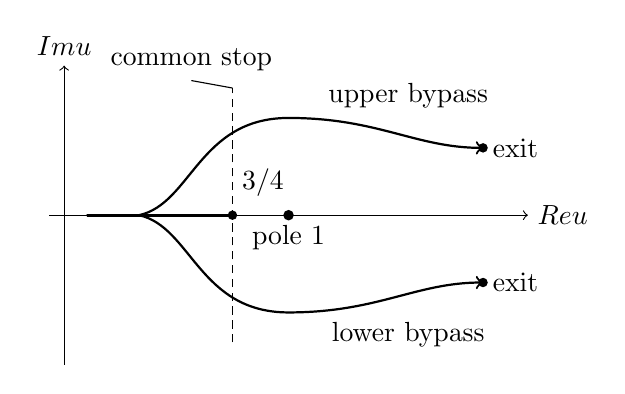
\begin{tikzpicture}[scale=0.95]
  \draw[->] (-0.2,0)--(6.2,0) node[right] {\(\operatorname{Re}u\)};
  \draw[->] (0,-2.0)--(0,2.0) node[above] {\(\operatorname{Im}u\)};
  \draw[densely dashed] (2.25,-1.7)--(2.25,1.7);
  \node[above right] at (2.25,0.12) {\(3/4\)};
  \fill (3,0) circle (2pt) node[below] {pole \(1\)};
  \draw[thick,->] (0.3,0)--(1.0,0)
    .. controls (1.7,0.15) and (1.8,1.3) .. (3.0,1.3)
    .. controls (4.2,1.3) and (4.7,0.9) .. (5.6,0.9);
  \draw[thick,->] (1.0,0)
    .. controls (1.7,-0.15) and (1.8,-1.3) .. (3.0,-1.3)
    .. controls (4.2,-1.3) and (4.7,-0.9) .. (5.6,-0.9);
  \draw[very thick] (0.3,0)--(2.25,0);
  \fill (2.25,0) circle (1.8pt);
  \node[above] (commonstop) at (1.7,1.8) {common stop};
  \draw[thin] (commonstop.south)--(2.25,1.7);
  \fill (5.6,0.9) circle (1.8pt) node[right] {exit};
  \fill (5.6,-0.9) circle (1.8pt) node[right] {exit};
  \node at (4.6,1.6) {upper bypass};
  \node at (4.6,-1.6) {lower bypass};
 \end{tikzpicture}
 \caption{Schematic only: the two bypasses can be curtailed and
 deformed to the thick real segment ending at the common pre-pole stop.
 The two artificial exits are marked.  The drawn curves are not
 the quantitative circle profiles; their admissibility is proved
 by \eqref{arr:circle-strict} and \eqref{arr:affine-homotopy}.}
 \label{arr:contour-schematic}
\end{figure}

Figure~\ref{arr:contour-schematic} shows the role of the common
pre-pole segment: curtailing both contour problems to that segment
allows uniqueness of the normalized solve to compare their actions.
